\section{Information extraction}
\label{sec:mem_extraction}







This component serves to identify and extract the information from $\mathcal{M}$ that is both useful and necessary for downstream memory processing.
As illustrated in Figure~\ref{fig:extraction}, existing agent systems adopt different information extraction methods, which can be broadly categorized as follows:


\begin{figure}[h]
\centering
\setlength{\abovecaptionskip}{0cm}
% \setlength{\belowcaptionskip}{-0.3cm}
\begin{AIbox}{Prompt for Summarization-based Extraction.}
{
\begin{tcolorbox}[colback=gray!10, colframe=gray!10, boxrule=0pt, sharp corners, left=0pt, right=0pt]
Generate a structured analysis of the following message by extracting salient keywords, identifying core themes and contextual elements, and assigning relevant categorical tags.

% 1. Identifying the most salient keywords (focus on nouns, verbs, and key concepts)

% 2. Extracting core themes and contextual elements

% 3. Creating relevant categorical tags

Format the response as a JSON object: 

{\ttfamily
\{
    
    {\hangindent=2em \hangafter=0 "summary": "<one-sentence gist>", \par}
        
        % {\hangindent=4em \hangafter=0 - Main topic/domain \par}
        
        % {\hangindent=4em \hangafter=0 - Key arguments/points \par}
        
        % {\hangindent=4em \hangafter=0 - Intended audience/purpose \par}
    
    \hspace*{2em}"keywords": [
    
        {\hangindent=4em \hangafter=0 <several keywords capturing key concepts> \par}

        % {\hangindent=4em \hangafter=0 - Order from most to least important. \par}
        
        % {\hangindent=4em \hangafter=0 - Don't include keywords that are the name of the speaker or time. \par}
        
        % {\hangindent=4em \hangafter=0 - At least three keywords, but don't be too redundant. \par}
                
    \hspace*{2em}],
    
    \hspace*{2em}"tags": [
    
        {\hangindent=4em \hangafter=0 <several broad themes for classification> \par}
        
        % {\hangindent=4em \hangafter=0 - Include domain, format, and type tags. \par}
        
        % {\hangindent=4em \hangafter=0 - At least three tags, but don't be too redundant. \par}
        
    \hspace*{2em}]
    
\}
}

Message for analysis:

\texttt{\{message\}}
\end{tcolorbox}
}
\end{AIbox}
\caption{A sample prompt for summarization-based extraction.}
\label{fig:pmt:summary_extract}
\end{figure}

\noindent {\Large \ding{182}} \textbf{Direct archiving.}
This method represents the most straightforward form of information extraction, where the agent system simply archives raw messages and timestamps without any processing. 







\noindent {\Large \ding{183}} \textbf{Summarization-based extraction.}
This method employs LLMs to generate concise informational summaries from one or more dialogue turns. Memory methods such as {\tt A-MEM} and {\tt Mem0} extract keywords and contextual tags from $\mathcal{M}$, or prompt the LLM to produce an abstracted summary of the raw text. Figure~\ref{fig:pmt:summary_extract} illustrates a representative prompt used for this extraction method.





\noindent {\Large \ding{184}} \textbf{Graph-based extraction.}
This method leverages LLMs to extract fine-grained entities and relations from $\mathcal{M}$, forming subject–predicate–object triples for knowledge graph construction (e.g., {\tt Mem0$^g$}, {\tt Zep}). Additionally, temporal metadata such as creation or invalidation timestamps are recorded to support dynamic updates and temporal reasoning within the graph-based memory. A concrete example of the prompt designed for graph-based extraction is provided in Appendix~\ref{sec:app:prompt}.


\begin{figure}[t]
    \centering
    \setlength{\abovecaptionskip}{0cm}
    % \setlength{\belowcaptionskip}{-0.3cm}
    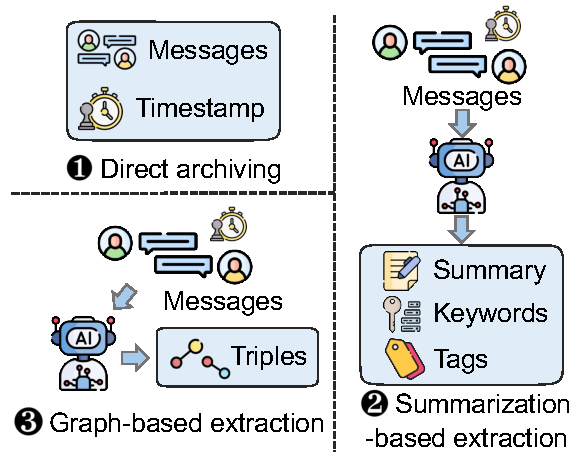
\includegraphics[width=0.7\linewidth]{figures/extraction.pdf}
    \caption{Methods of information extraction.}
    \label{fig:extraction}
\end{figure}